% GNUPLOT: LaTeX picture with Postscript
\begingroup
  \makeatletter
  \providecommand\color[2][]{%
    \GenericError{(gnuplot) \space\space\space\@spaces}{%
      Package color not loaded in conjunction with
      terminal option `colourtext'%
    }{See the gnuplot documentation for explanation.%
    }{Either use 'blacktext' in gnuplot or load the package
      color.sty in LaTeX.}%
    \renewcommand\color[2][]{}%
  }%
  \providecommand\includegraphics[2][]{%
    \GenericError{(gnuplot) \space\space\space\@spaces}{%
      Package graphicx or graphics not loaded%
    }{See the gnuplot documentation for explanation.%
    }{The gnuplot epslatex terminal needs graphicx.sty or graphics.sty.}%
    \renewcommand\includegraphics[2][]{}%
  }%
  \providecommand\rotatebox[2]{#2}%
  \@ifundefined{ifGPcolor}{%
    \newif\ifGPcolor
    \GPcolortrue
  }{}%
  \@ifundefined{ifGPblacktext}{%
    \newif\ifGPblacktext
    \GPblacktexttrue
  }{}%
  % define a \g@addto@macro without @ in the name:
  \let\gplgaddtomacro\g@addto@macro
  % define empty templates for all commands taking text:
  \gdef\gplbacktext{}%
  \gdef\gplfronttext{}%
  \makeatother
  \ifGPblacktext
    % no textcolor at all
    \def\colorrgb#1{}%
    \def\colorgray#1{}%
  \else
    % gray or color?
    \ifGPcolor
      \def\colorrgb#1{\color[rgb]{#1}}%
      \def\colorgray#1{\color[gray]{#1}}%
      \expandafter\def\csname LTw\endcsname{\color{white}}%
      \expandafter\def\csname LTb\endcsname{\color{black}}%
      \expandafter\def\csname LTa\endcsname{\color{black}}%
      \expandafter\def\csname LT0\endcsname{\color[rgb]{1,0,0}}%
      \expandafter\def\csname LT1\endcsname{\color[rgb]{0,1,0}}%
      \expandafter\def\csname LT2\endcsname{\color[rgb]{0,0,1}}%
      \expandafter\def\csname LT3\endcsname{\color[rgb]{1,0,1}}%
      \expandafter\def\csname LT4\endcsname{\color[rgb]{0,1,1}}%
      \expandafter\def\csname LT5\endcsname{\color[rgb]{1,1,0}}%
      \expandafter\def\csname LT6\endcsname{\color[rgb]{0,0,0}}%
      \expandafter\def\csname LT7\endcsname{\color[rgb]{1,0.3,0}}%
      \expandafter\def\csname LT8\endcsname{\color[rgb]{0.5,0.5,0.5}}%
    \else
      % gray
      \def\colorrgb#1{\color{black}}%
      \def\colorgray#1{\color[gray]{#1}}%
      \expandafter\def\csname LTw\endcsname{\color{white}}%
      \expandafter\def\csname LTb\endcsname{\color{black}}%
      \expandafter\def\csname LTa\endcsname{\color{black}}%
      \expandafter\def\csname LT0\endcsname{\color{black}}%
      \expandafter\def\csname LT1\endcsname{\color{black}}%
      \expandafter\def\csname LT2\endcsname{\color{black}}%
      \expandafter\def\csname LT3\endcsname{\color{black}}%
      \expandafter\def\csname LT4\endcsname{\color{black}}%
      \expandafter\def\csname LT5\endcsname{\color{black}}%
      \expandafter\def\csname LT6\endcsname{\color{black}}%
      \expandafter\def\csname LT7\endcsname{\color{black}}%
      \expandafter\def\csname LT8\endcsname{\color{black}}%
    \fi
  \fi
  \setlength{\unitlength}{0.0500bp}%
  \begin{picture}(7200.00,5040.00)%
    \gplgaddtomacro\gplbacktext{%
      \csname LTb\endcsname%
      \put(1188,704){\makebox(0,0)[r]{\strut{}$-0.03$}}%
      \put(1188,1156){\makebox(0,0)[r]{\strut{}$-0.02$}}%
      \put(1188,1609){\makebox(0,0)[r]{\strut{}$-0.01$}}%
      \put(1188,2061){\makebox(0,0)[r]{\strut{}$0$}}%
      \put(1188,2514){\makebox(0,0)[r]{\strut{}$0.01$}}%
      \put(1188,2966){\makebox(0,0)[r]{\strut{}$0.02$}}%
      \put(1188,3419){\makebox(0,0)[r]{\strut{}$0.03$}}%
      \put(1188,3871){\makebox(0,0)[r]{\strut{}$0.04$}}%
      \put(1188,4324){\makebox(0,0)[r]{\strut{}$0.05$}}%
      \put(1188,4776){\makebox(0,0)[r]{\strut{}$0.06$}}%
      \put(1320,484){\makebox(0,0){\strut{}$0$}}%
      \put(1864,484){\makebox(0,0){\strut{}$1$}}%
      \put(2408,484){\makebox(0,0){\strut{}$2$}}%
      \put(2952,484){\makebox(0,0){\strut{}$3$}}%
      \put(3496,484){\makebox(0,0){\strut{}$4$}}%
      \put(4040,484){\makebox(0,0){\strut{}$5$}}%
      \put(4584,484){\makebox(0,0){\strut{}$6$}}%
      \put(5128,484){\makebox(0,0){\strut{}$7$}}%
      \put(5672,484){\makebox(0,0){\strut{}$8$}}%
      \put(6216,484){\makebox(0,0){\strut{}$9$}}%
      \put(6760,484){\makebox(0,0){\strut{}$10$}}%
      \put(286,2740){\rotatebox{-270}{\makebox(0,0){\strut{}$g_6(r)$}}}%
      \put(6979,2740){\rotatebox{-270}{\makebox(0,0){\strut{}}}}%
      \put(4040,154){\makebox(0,0){\strut{}$r/\sigma$}}%
      \put(4040,4666){\makebox(0,0){\strut{}}}%
      \put(4040,4665){\makebox(0,0){\strut{}}}%
      \put(132,110){\makebox(0,0)[l]{\strut{}}}%
    }%
    \gplgaddtomacro\gplfronttext{%
      \csname LTb\endcsname%
      \put(5773,1922){\makebox(0,0)[r]{\strut{}$\phi=0.497$}}%
      \csname LTb\endcsname%
      \put(5773,1592){\makebox(0,0)[r]{\strut{}$\phi=0.535$}}%
      \csname LTb\endcsname%
      \put(5773,1262){\makebox(0,0)[r]{\strut{}$\phi=0.555$}}%
      \csname LTb\endcsname%
      \put(5773,932){\makebox(0,0)[r]{\strut{}$\phi=0.576$}}%
    }%
    \gplgaddtomacro\gplbacktext{%
      \csname LTb\endcsname%
      \put(3348,3071){\makebox(0,0)[r]{\strut{}$10^{-5}$}}%
      \put(3348,3798){\makebox(0,0)[r]{\strut{}$10^{-3}$}}%
      \put(3348,4524){\makebox(0,0)[r]{\strut{}$10^{-1}$}}%
      \put(4026,2488){\makebox(0,0){\strut{}$2$}}%
      \put(4619,2488){\makebox(0,0){\strut{}$4$}}%
      \put(5213,2488){\makebox(0,0){\strut{}$6$}}%
      \put(5806,2488){\makebox(0,0){\strut{}$8$}}%
      \put(6400,2488){\makebox(0,0){\strut{}$10$}}%
      \put(6619,3616){\rotatebox{-270}{\makebox(0,0){\strut{}}}}%
      \put(4940,4414){\makebox(0,0){\strut{}}}%
      \put(4940,4413){\makebox(0,0){\strut{}}}%
      \put(2028,2378){\makebox(0,0)[l]{\strut{}}}%
    }%
    \gplgaddtomacro\gplfronttext{%
    }%
    \gplbacktext
    \put(0,0){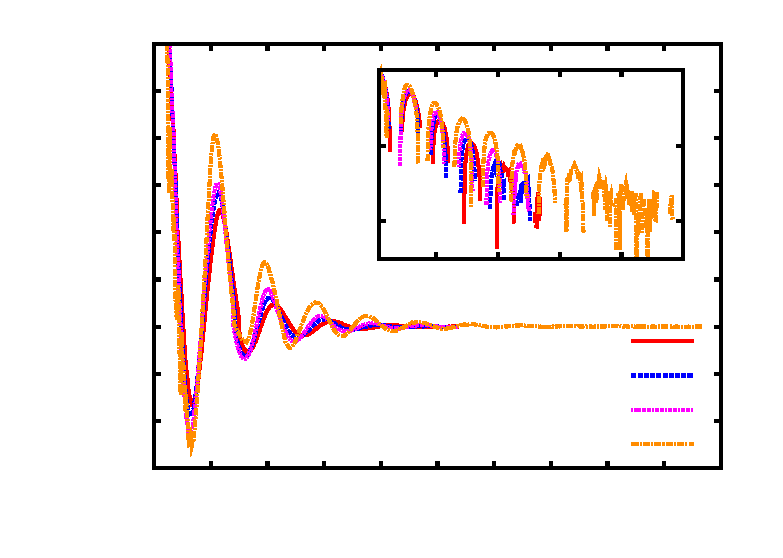
\includegraphics{g6}}%
    \gplfronttext
  \end{picture}%
\endgroup
